\chapter{\ifproject%
\ifenglish Project Structure and Methodology\else โครงสร้างและขั้นตอนการทำงาน\fi
\else%
\ifenglish Project Structure\else โครงสร้างของโครงงาน\fi
\fi
}

ในบทนี้จะกล่าวถึงหลักการ และการออกแบบระบบ

\makeatletter

% \renewcommand\section{\@startsection {section}{1}{\z@}%
%                                    {13.5ex \@plus -1ex \@minus -.2ex}%
%                                    {2.3ex \@plus.2ex}%
%                                    {\normalfont\large\bfseries}}

\makeatother
%\vspace{2ex}
% \titleformat{\section}{\normalfont\bfseries}{\thesection}{1em}{}
% \titlespacing*{\section}{0pt}{10ex}{0pt}

\section{โครงสร้างของเว็บไซต์}
โปรเจคนี้จะแบ่งออกเป็น 3 ส่วน
\begin{enumerate}
  \item Fontend - ใช้ React ในการจัดการหน้าเว็ปไซต์
  \item Backend - ใช้ Nest เป็นตัวกลางในการสื่อสารระหว่าง Fontend และ Database ด้วย API
  \item Database - ใช้การเก็บข้อมูลแบบ SQL โดยใช้ PostgreSQL และใช้ Firebase Cloud Storage ในการเก็บรูปภาพจากการอัพโหลด
\end{enumerate}


\begin{figure}[h]
  \begin{center}
  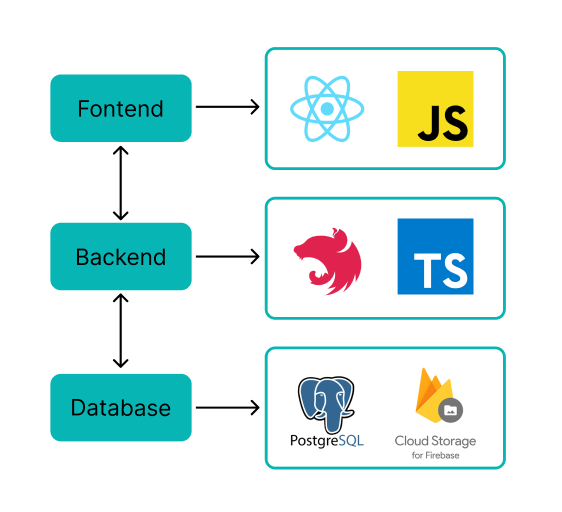
\includegraphics[width=6cm,height=6cm,keepaspectratio]{SWA.png}
  \end{center}
  \caption[โครงสร้างของเว็บไซต์]{โครงสร้างของเว็บไซต์}
  \label{fig:โครงสร้างของเว็บไซต์}
\end{figure}

\section{ฟีเจอร์}
\subsection{ฟีเจอร์การใช้งานของผู้เล่น}
การใช้งานในฝั่งผู้เล่นจะมีระบบหลักๆ ดังนี้
\begin{enumerate}
  \item ระบบสร้างทีม - ใช้สร้างทีมเพื่อเข้าร่วมการแข่งขันทัวร์นาเมนต์ต่างๆ โดยจะสร้างทีมเป็นของแต่ละเกมที่ต้องการแข่งแยกกัน เช่น ทีมValorant ก็จะใช้ลงทัวร์นาเมนต์ได้แค่เกม Valorant เท่านั้น
  \item ระบบจัดการทีม - ใช้จัดการในการเปลี่ยนชื่อ จัดการคนในทีม รับคนเข้าทีม และแสดงประวัติการเล่นของทีม
  \item ระบบจัดการโปรไฟล์ - ใช้จัดการโปรไฟล์เปลี่ยนชื่อ แสดงข้อมูลการเข้าร่วมแข่ง และทีมที่อยู่
  \item ระบบเลือก และสมัครทัวร์นาเมนต์ - เลือกทัวร์นาเมนต์ที่ต้องการแข่งขั้นสามารถดูรายละเอียด เลือกเกมที่ต้องการ และสมัครเข้าร่วมการแข่งขันได้
\end{enumerate}

\subsection{ฟีเจอร์การใช้งานของผู้จัดงาน}
การใช้งานในฝั่งผู้จัดการจะมีระบบหลักๆ ดังนี้
\begin{enumerate}
  \item ระบบสร้างจัดการทัวร์นาเมนต์ - ใช้สร้างทัวร์นาเมต์กำหนดรายระเอียดการแข่ง กฎกติกา เวลาแข่ง และรูปหน้าปกทัวร์นาเมนต์
  \item ระบบเดชบอร์ดในการจัดการทัวร์นาเมนต์ - ใช้ในการจัดการทัวร์นาเมนต์ผลแพ้ชนะ และเช็คหลักฐานการแข่งของแต่ละทีม
  \item ระบบจัดตารางแข่ง - โดยระบบจะนำผู้เล่นที่มาสมัครเข้าทัวร์นาเมนต์นั้นๆมาสุ่มเรียงเข้าตารางให้ และอัพเดตตารางการแข่งขันเมื่อผลการแข่งขันมีการปรับเปลี่ยน
\end{enumerate}

\begin{figure}[h]
  \begin{center}
  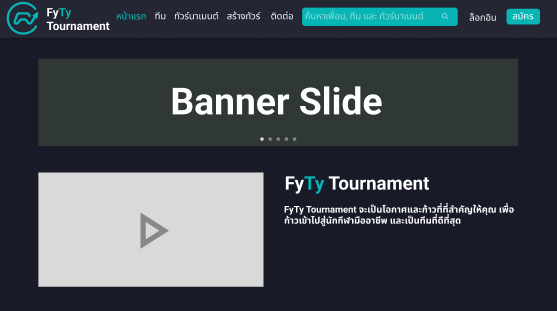
\includegraphics[width=10cm,height=6cm,keepaspectratio]{homebf.png}
  \end{center}
  \caption[หน้าแรกของระบบที่ยังไม่ได้ล็อกอิน]{หน้าแรกของระบบที่ยังไม่ได้ล็อกอิน}
  \label{fig:หน้าแรกของระบบที่ยังไม่ได้ล็อกอิน}
\end{figure}

\begin{figure}[h]
  \begin{center}
  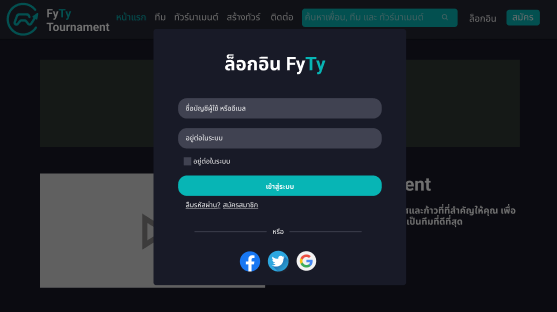
\includegraphics[width=10cm,height=6cm,keepaspectratio]{login.png}
  \end{center}
  \caption[หน้าล็อกอิน]{หน้าล็อกอิน}
  \label{fig:หน้าล็อกอิน}
\end{figure}

\begin{figure}[h]
  \begin{center}
  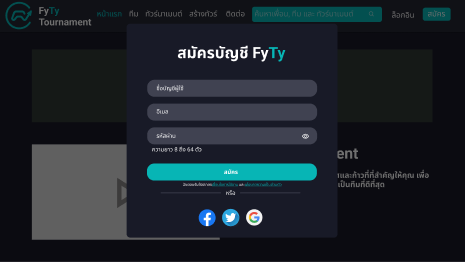
\includegraphics[width=10cm,height=6cm,keepaspectratio]{reg.png}
  \end{center}
  \caption[หน้าสมัคร]{หน้าสมัคร}
  \label{fig:หน้าสมัคร}
\end{figure}

\begin{figure}[h]
  \begin{center}
  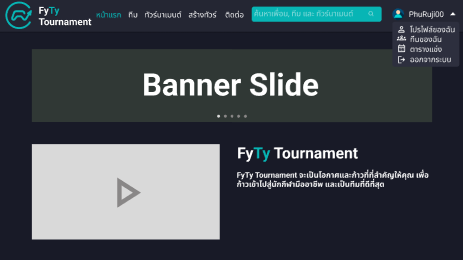
\includegraphics[width=10cm,height=6cm,keepaspectratio]{homeaf.png}
  \end{center}
  \caption[หน้าแรกของระบบหลังล็อกอิน]{หน้าแรกของระบบหลังล็อกอิน}
  \label{fig:หน้าแรกของระบบหลังล็อกอิน}
\end{figure}

\begin{figure}[h]
  \begin{center}
  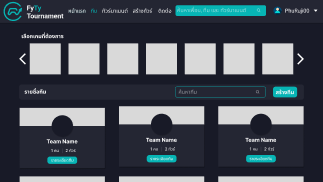
\includegraphics[width=10cm,height=6cm,keepaspectratio]{allteam.png}
  \end{center}
  \caption[หน้าทีมทั้งหมด]{หน้าทีมทั้งหมด}
  \label{fig:หน้าทีมทั้งหมด}
\end{figure}

\begin{figure}[h]
  \begin{center}
  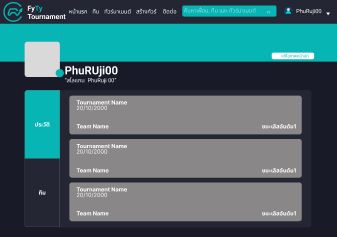
\includegraphics[width=10cm,height=6cm,keepaspectratio]{profileHis.png}
  \end{center}
  \caption[หน้าโปรไฟล์(ประวัติ)]{หน้าโปรไฟล์(ประวัติ)}
  \label{fig:หน้าโปรไฟล์(ประวัติ)}
\end{figure}

\begin{figure}[h]
  \begin{center}
  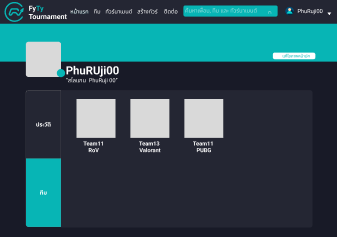
\includegraphics[width=10cm,height=6cm,keepaspectratio]{profileTeam.png}
  \end{center}
  \caption[หน้าโปรไฟล์(ทีม)]{หน้าโปรไฟล์(ทีม)}
  \label{fig:หน้าโปรไฟล์(ทีม)}
\end{figure}

\begin{figure}[h]
  \begin{center}
  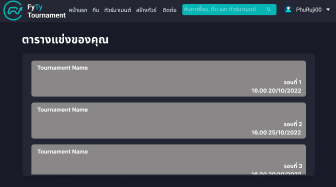
\includegraphics[width=10cm,height=6cm,keepaspectratio]{schedule.png}
  \end{center}
  \caption[ตารางแข่ง]{ตารางแข่ง}
  \label{fig:ตารางแข่ง}
\end{figure}

\begin{figure}[h]
  \begin{center}
  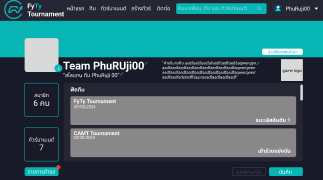
\includegraphics[width=10cm,height=10cm,keepaspectratio]{teamDetail.png}
  \end{center}
  \caption[หน้ารายละเอียดทีม และจัดการทีม]{หน้ารายละเอียดทีม และจัดการทีม}
  \label{fig:หน้ารายละเอียดทีม และจัดการทีม}
\end{figure}

\begin{figure}[h]
  \begin{center}
  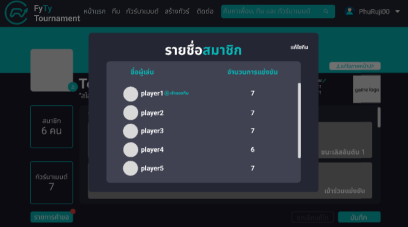
\includegraphics[width=10cm,height=10cm,keepaspectratio]{member.png}
  \end{center}
  \caption[หน้ารายละเอียดทีม และจัดการทีม(สมาชิกทีม)]{หน้ารายละเอียดทีม และจัดการทีม(สมาชิกทีม)}
  \label{fig:หน้ารายละเอียดทีม และจัดการทีม(สมาชิกทีม)}
\end{figure}

\begin{figure}[h]
  \begin{center}
  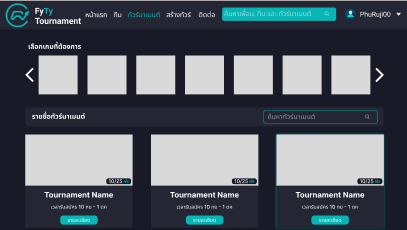
\includegraphics[width=10cm,height=6cm,keepaspectratio]{allTour.png}
  \end{center}
  \caption[หน้าทัวร์นาเมนต์ทั้งหมด]{หน้าทัวร์นาเมนต์ทั้งหมด}
  \label{fig:หน้าทัวร์นาเมนต์ทั้งหมด}
\end{figure}

\begin{figure}[h]
  \begin{center}
  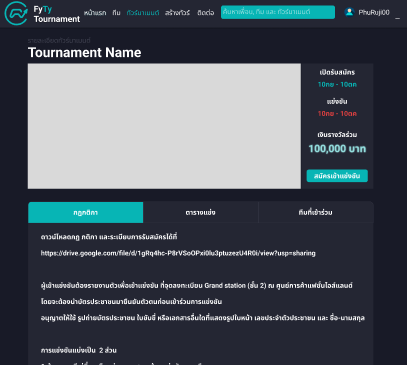
\includegraphics[width=10cm,height=10cm,keepaspectratio]{tourRule.png}
  \end{center}
  \caption[หน้ารายละเอียดทัวร์นาเมนต์(กฎกติกา)]{หน้ารายละเอียดทัวร์นาเมนต์(กฎกติกา)}
  \label{fig:หน้ารายละเอียดทัวร์นาเมนต์(กฎกติกา)}
\end{figure}

\begin{figure}[h]
  \begin{center}
  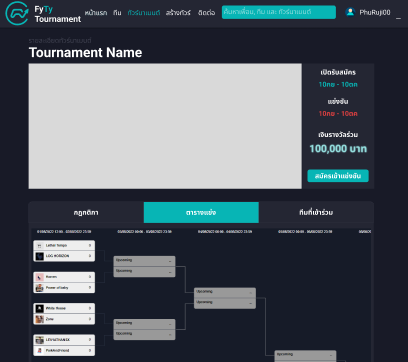
\includegraphics[width=10cm,height=10cm,keepaspectratio]{tourBac.png}
  \end{center}
  \caption[หน้ารายละเอียดทัวร์นาเมนต์(ตารางแข่ง)]{หน้ารายละเอียดทัวร์นาเมนต์(ตารางแข่ง)}
  \label{fig:หน้ารายละเอียดทัวร์นาเมนต์(ตารางแข่ง)}
\end{figure}

\begin{figure}[h]
  \begin{center}
  \includegraphics[width=10cm,height=10cm,keepaspectratio]{TourTeam.png}
  \end{center}
  \caption[หน้ารายละเอียดทัวร์นาเมนต์(ทีมที่สมัคร)]{หน้ารายละเอียดทัวร์นาเมนต์(ทีมที่สมัคร)}
  \label{fig:หน้ารายละเอียดทัวร์นาเมนต์(ทีมที่สมัคร)}
\end{figure}

\begin{figure}[h]
  \begin{center}
  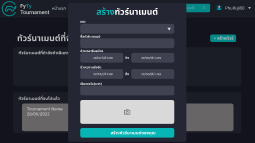
\includegraphics[width=10cm,height=6cm,keepaspectratio]{createtournament.png}
  \end{center}
  \caption[หน้าสร้างทัวร์นาเมนต์]{หน้าสร้างทัวร์นาเมนต์}
  \label{fig:หน้าสร้างทัวร์นาเมนต์}
\end{figure}

\begin{figure}[h]
  \begin{center}
  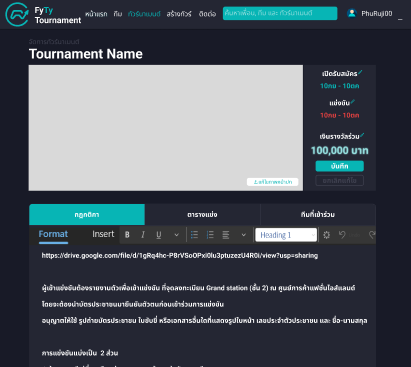
\includegraphics[width=10cm,height=10cm,keepaspectratio]{createDetail.png}
  \end{center}
  \caption[หน้าจัดการรายละเอียดทัวร์นาเมนต์]{หน้าจัดการรายละเอียดทัวร์นาเมนต์}
  \label{fig:หน้าจัดการรายละเอียดทัวร์นาเมนต์}
\end{figure}

\begin{figure}[h]
  \begin{center}
  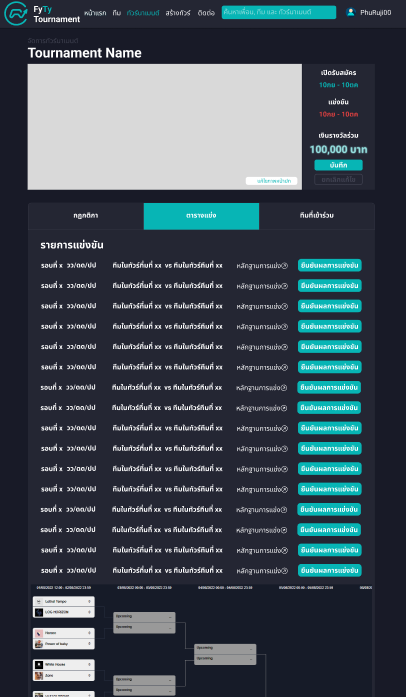
\includegraphics[width=10cm,height=15cm,keepaspectratio]{dashbordTour.png}
  \end{center}
  \caption[หน้าทัวร์นาเมนต์แดชบอร์ด]{หน้าทัวร์นาเมนต์แดชบอร์ด}
  \label{fig:หน้าทัวร์นาเมนต์แดชบอร์ด}
\end{figure}
